\documentclass[12pt]{scrreprt}

\usepackage[onehalfspacing]{setspace}

\usepackage[utf8]{inputenc}
\usepackage{ngerman}

\usepackage{amsmath}
\usepackage{amssymb}

\usepackage{listings}
\usepackage[usenames,dvipsnames]{color}
\usepackage{graphicx} 

\lstloadlanguages{Ruby}
\lstset{basicstyle=\ttfamily\color{black}, commentstyle = \ttfamily\color{grey}, keywordstyle=\ttfamily\color{Violet}, stringstyle=\color{blue}, breaklines=true, showstringspaces=false}

\begin{document}

%\tableofcontents \newpage
  
\chapter{Punkteberechnung (verfasst von Thomas Eger)}

\section{Aufgabenstellung}

Innerhalb der existierenden Web-Anwendung zur administrativen Unterstützung der verschiedenen o/ZB wird ein Mechanismus benötigt, der dafür zuständig ist, die für Kontenbewegungen entstehenden Punkte zu ermitteln. Die Berechnungen dazu sind im bestehenden System redundant implementiert. \\

Dieser Teil der Projektarbeit dokumentiert das Refactoring zur Zusammenfassung dieser Berechnungen, die dabei entstandenen Programmteile, sowie deren Verwendung. 

\section{Fachliche Erläuterungen}
Zunächst sollen einige fachliche Erläuterungn einen einfacheren Einstieg in die Programmierung ermöglichen.  

\subsection{Überblick über das Punktesystem der o/ZB}
Für das Ansparen werden statt Zinsen sogenannte Sparpunkte vergeben. Das Sparen findet in zeitlich begrenzten Phasen statt, in denen beispielsweise monatlich über ein Jahr ein bestimmter Währungs-Betrag angelegt wird. Nach Ablauf einer solchen Ansparphase kann das Währungs-Guthaben wieder entnommen werden. Die Sparpunkte bleiben auf dem Konto. \\

Wenn das angesparte Guthaben nicht für das umzusetzende Projekt ausreicht kann eine Zusatzentnahme erfolgen. Dies entspricht in etwa einem Darlehen auf der Bank. Entsprechend der Vergabe von Punkten beim Ansparen, muss der Darlehensnehmer genügend Sparpunkte angesammelt haben, damit eine Zusatzentnahme möglich wird. Es besteht auch die Möglichkeit Punkte zu leihen oder zu schenken. \\

Um in der Web-Anwendung die Punkte korrekt darstellen zu können, bedarf es einer Formel zu deren Berechnung über eine gegebene Zeitspanne, mit einem gegebenen Wäh{"-}rungs-Betrag. \\

\begin{table}
  \begin{center}
    \begin{tabular}{|l|r|}
      \hline
      \textbf{Kontenklasse} & \textbf{Faktor}\\
      \hline
      A & 1,0\\
      \hline
      B & 0,75\\
      \hline
      C & 0,5\\
      \hline
      D & 0,25\\
      \hline
      E & 0,0\\
      \hline
    \end{tabular}
    \caption{Vorhandene Kontenklassen}
    \label{kkl}
  \end{center}
\end{table}
\vspace{2mm}

Weitere Parameter für die Berechnung ergeben sich aus dem Kontenklassenverlauf eines o/ZB-Mitglieds. Jedes Mitglied befindet sich zu jeder Zeit in einer Kontenklasse, die auch gewechselt werden kann. Der zeitliche Ablauf der Kontenklassenwechsel heisst Kontenklassenverlauf. Jeder Klasse ist ein Faktor zugeordnet. Die Kontenklassen in Tabelle \ref{kkl} existieren zur Zeit dieser Projektarbeit. \\

\subsection{Berechnung der Punkte}
Die folgende Formel dient zur Berechnung der Punkte für einen einzelnen Währungs-Betrag über mehrere Kontenklassen.

\begin{equation*}
  Punkte = \sum_{i=0}^{K} \frac{t_i}{30} * k_i * w
\end{equation*}

\begin{align*}
 K &= \text{Anzahl der Kontenklassenwechsel} \\
 i &= \text{Index der momentanen Kontenklasse} \\
 k_i &= \text{Faktor der momentanen Kontenklasse} \\
 t_i &= \text{Anzahl Tage innerhalb der momentanen Kontenklasse} \\
 w &= \text{Währungs-Betrag} 
\end{align*}

Es muss über die Kontenklassen innerhalb einer gegebenen Zeitspanne iteriert werden. Dabei werden in jedem Schritt die Anzahl der Tage mit dem Kontenklassenfaktor und dem Währungs-Betrag multipliziert. Die Summe der Teilergebnisse bildet die Punkte über die gegebene Zeitspanne mit dem gegebenen Währungs-Betrag. Die Division durch 30 dient als Skalierung für die tagesgenaue Berechnung der Punkte innerhalb von Monaten. Das folgende Beispiel soll die Anwendung der Formel verdeutlichen.

\subsubsection{Beispiel}
Es sollen die Punkte für das Konto 70013 im Zeitraum vom 15.07.2008 bis zum 05.08.2008 berechnet werden. Der Saldo auf diesem Konto beträgt 1000,0 Euro. Der dazugehörige Kontenklassenverlauf steht in Tabelle \ref{kklverlauf}.

\begin{table}
  \begin{center}
    \begin{tabular}{|l|r|r|}
      \hline
      \textbf{Kontenklasse} & \textbf{Faktor} & \textbf{Startdatum}\\
      \hline
      A & 1,0 & 01.01.2005\\
      \hline
      B & 0,75 & 01.01.2008\\
      \hline
      C & 0,5 & 01.08.2008\\
      \hline
      B & 0,75 & 01.01.2009\\
      \hline
    \end{tabular}
    \caption{Kontenklassenverlauf für das Konto 70013}
    \label{kklverlauf}
  \end{center}
\end{table}
\vspace{2mm}

Vom 15.07.2008 bis 31.07.2008 sind es 16 Tage in Kontenklasse B, vom 01.08.2008 bis 05.08.2008 sind es  5 Tage in Kontenklasse C. Jetzt lassen sich alle Parameter in die Formel einsetzen:

\begin{equation*}
  Punkte = \left(\frac{16}{30} * 0,75 * 1000,0\right) + \left(\frac{5}{30} * 0,5 * 1000,0\right) = 400,0 + 83,33 = 483,33
\end{equation*} \\

Um nun die Punkte für einen Kontoauszug wie in Abbildung \ref{account} berechnen zu können muss eine erweiterte Formel verwendet werden, die die vorher erläuterte verwendet und für verschiedene Zeiträume und Währungs-Beträge aufruft. 

\begin{equation*}
  PunkteEndsaldo = PunkteAnfangssaldo + \sum_{j=1}^{I} \left(\sum_{i=0}^{K} \frac{t_{ij}}{30} * k_{ij} * w_i\right)
\end{equation*}

\begin{align*}
 K &= \text{Anzahl der Kontenklassenwechsel} \\
 I &= \text{Anzahl der Zeitintervalle} \\
 j &= \text{Index der momentanen Kontenklasse} \\
 i &= \text{Index für den momentanen Zeitintervall} \\
 k_{ij} &= \text{Faktor der momentanen Kontenklasse im aktuellen Zeitintervall} \\
 t_{ij} &= \text{Anzahl Tage innerhalb der momentanen Kontenklasse im aktuellen Zeitintervall} \\
 w_i &= \text{Währungs-Betrag im aktuellen Zeitintervall} 
\end{align*}

Mit der erweiterten Formel kann nun der Tagessaldo in Abbildung \ref{account} berechnet werden. Dazu wird über alle Einträge in der Liste iteriert (äußere Summe in der Formel) und die Punkteberechnung zwischen dem vorherigen Datum und dem aktuellen Datum berechnet. Das Ergebnis wird auf den vorherigen PunkteAnfangssaldo addiert bis alle Buchungen im gegebenen Zeitraum abgearbeitet sind. Der Tagessaldo entspricht dann dem PuntkeEndsaldo aus der erweiterten Formel. \\

\begin{figure} 
  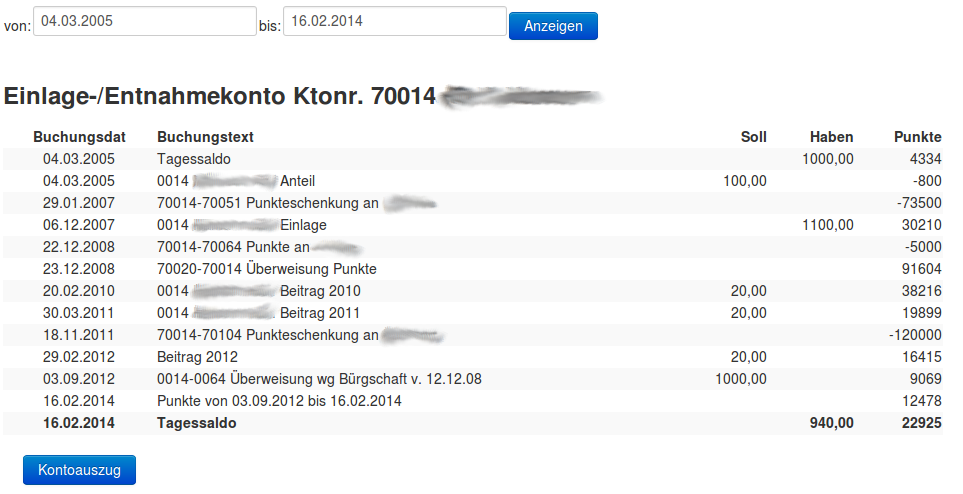
\includegraphics[width=\textwidth]{account-ano.png}
  \caption{Beispiel eines Kontoauszugs im Produktivsystem. Die Namen wurden geschwärzt.}
  \label{account}
\end{figure}

Des Weiteren soll das Vorgehen bei der Implementierung einer Klasse betrachtet werden, die alle Anforderungen an die Punkteberechnung erfüllt. Zunächst wird hierfür die bestehende Umsetzung betrachtet, Probleme aufgezeigt und danach eine Lösung erarbeitet und umgesetzt.

\newpage

\section{Analyse der alten Implementierung}
Bei einer genauen Betrachtung der alten Implementierung fällt auf, dass die Punkteberechnung an jeder notwendigen Stelle separat und teilweise auf unterschiedliche Weise umgesetzt ist. Das führt dazu, dass das Programm fehleranfällig und sehr schwer wartbar ist. Falls ein Fehler gefunden wird, muss dieser an vielen verschiedenen Stellen separat behoben werden. Außerdem gibt es bei einer redundanten Implementierung keine Möglichkeit Modul-Tests einzusetzen, da kein einzelnes zu testendes Modul existiert, sondern viele verschiedene. \\

Gerade bei Programmteilen, die essentiell für die Geschäftslogik sind, ist es unabdingbar Modul-Tests für die Verifikation der fachlichen Korrektheit einzusetzen. Diese bieten die Sicherheit, dass zum Beispiel die Ergebnisse einer Berechnung stimmen und können nach jeder Änderung am betreffenden Modul ausgeführt werden. So fallen Unstimmigkeiten dem Programmierer sofort auf und können behoben werden. \\ 

Die Stellen, an denen eine Nummerierung statt gefunden hat sind in Tabelle \ref{redundant} aufgelistet. Alle Dateinamen sind relativ zum Wurzelordner der Rails-Anwendung. Ein Controller-Test, der die berechneten Werte, die an die Oberfläche übergeben werden, überprüft, existiert bereits in der Datei 
\newline \verb+spec/controllers/DarlehensverlaufController_spec.rb+.

\begin{table}
  \begin{center}
    \begin{tabular}{|l|r|}
      \hline
      \textbf{Dateiname} & \textbf{Zeile}\\
      \hline
      controllers/darlehensverlauf\_controller.rb & 80\\
      \hline
      controllers/darlehensverlauf\_controller.rb & 99\\
      \hline
      controllers/darlehensverlauf\_controller.rb & 137\\
      \hline
      controllers/darlehensverlauf\_controller.rb & 167\\
      \hline
      controllers/darlehensvertrag\_controller.rb & ab 104\\
      \hline
      controllers/webimport\_controller.rb & 264\\
      \hline
      spec/controllers/DarlehensverlaufController\_spec.rb & ab 36\\
      \hline
    \end{tabular}
    \caption{Redundante Stellen im Quelltext}
    \label{redundant}
  \end{center}
\end{table}
\vspace{2mm}

\section{Anforderungen}
Aus der Analyse der alten Implementierung ergeben sich folgende Anforderungen.

\subsection{Zentrale Punkteberechnung}
Mit Hilfe der Implementierung einer zentralen Klasse, die alle benötigten Methoden zur Verfügung stellt um die Punkteberechnung durchzuführen, sollen die vielen redundanten Berechnungen durch eine einheitliche ersetzt werden. Dazu ist lediglich eine nach außen sichtbare Funktion von Nöten, die die Berechnung so durchführt, dass sie der vorher beschriebenen Formel entspricht. Der benutzer der Methode soll keine eigenen Datenbankabfragen durchführen müssen. Dazu sind folgende Parameter notwendig:

\begin{itemize}
  \item Das \emph{Startdatum} für die zu berechnende Zeitspanne
  \item Das \emph{Enddatum} für die zu berechnende Zeitspanne
  \item Der \emph{Währungs-Betrag} (Saldo) für die zu berechnende Zeitspanne
  \item Die \emph{Kontonummer} für das betroffene Konto. Sie wird benötigt, um den Kontenklassenverlauf für die betroffene Zeitspanne aus der Datenbank zu ermitteln
  \item Ein boolscher Wert, der bestimmt, ob das Ergebnis \emph{gerundet} werden soll, oder nicht. Standardmäßig soll keine Rundung erfolgen
\end{itemize}

\subsection{Spezifikation der Testfälle}
Außer der eigentlichen Berechnung soll ein Modul-Test implementiert werden, der die korrekte fachliche Umsetzung der Berechnung sicherstellt. Dabei müssen auch eventuelle Hilfsfunktionen getestet werden. So ergeben sich folgende Testfälle:

\begin{itemize}
  \item Berechnung der Punkte für einen gegebenen Zeitraum, Währungs-Betrag und Kontonummer
  \item Berechnung der Punkte für einen gegebenen Zeitraum, Währungs-Betrag und Kontonummer ohne, dass gerundet werden soll
  \item Ermittlung der im Zeitraum betroffenen Kontenklassen
  \item Ermittlung der Anzahl von Tagen in einer Kontenklasse
  \item Berechnung des Faktors für eine Kontenklasse
  \item Berechnung der Anzahl von Tagen zwischen zwei Daten
  \item Berechnung der Anzahl von Tagen zwischen zwei Daten in einem Schaltjahr  
\end{itemize}

\section{Realisierung}

Da nun die Testfälle spezifiziert sind, kann nach dem Test-Driven-Development Model mit der Realisierung des Refactorings begonnen werden. In diesem Abschnitt werden die entstandenen Methoden und dazugehörigen Tests genauer dokumentiert.

\subsection{Die Klasse Punkteberechnung}

Implementiert ist die Klasse Punkteberechnung in der Datei \newline\verb+lib/Punkte/Punkteberechnung.rb+. Die Methoden der Klasse werden im Folgenden erläutert.\\

\begin{lstlisting}[language=Ruby]
def self.calculate(date_begin, date_end, amount, account_number, round_down = true)
\end{lstlisting}
Die zentrale Methode der Punkteberechnung ist \verb+calculate+. Sie bekommt vom Aufrufer die bereits beschriebenen Parameter übergeben und leitet sie an die nächste Methode weiter. Eine Besonderheit ist hierbei \verb+round_down+. Dieser ist standardmäßig auf \verb+true+ gesetzt, was dazu führt, dass der Aufrufer diesen Wert nicht explizit angeben muss. Falls die Rundung nicht erwünscht ist kann hier \verb+false+ übergeben werden. \\

\begin{lstlisting}[language=Ruby]
def self.calc_score_new(date_begin, date_end, amount, account_number)
\end{lstlisting}
Diese Methode berechnet den eigentlichen Punktestand und gibt diesen ungerundet zurück. Dabei werden intern die Methoden \verb+get_affected_account_class_changes+, \verb+get_days_in_account_classes+ und \verb+get_factor_for_account_class+ genutzt, um die für die Berechnung  notwendigen Daten zu ermitteln. Dabei wird über die Map \newline\verb+days_in_account_classes+ iteriert und die jeweils berechneten Punkte summiert. Dies entspricht der Implementierung der vorher beschriebenen Formel zur Punkteberechnung. \\

\begin{lstlisting}[language=Ruby]
def self.get_factor_for_account_class(account_class) 
\end{lstlisting}
Wie schon beschrieben, ist jeder Kontenklasse ein Faktor zugeordnet. Diese Methode bekommt als Parameter ein Objekt vom Typ Kontenklasse (KKL) übergeben, liest dort den Prozentsatz aus und teilt diesen durch 100. So kann der Faktor direkt in der Formel verrechnet werden. \\

\begin{lstlisting}[language=Ruby]
def self.get_affected_account_class_changes(date_begin, date_end, account_number)
\end{lstlisting}
Laut den Anforderungen soll es nicht nötig sein, dass der Aufrufer der Punkteberechnung auf die Datenbank zugreift. Diese Aufgabe übernimmt diese Methode. Sie ermittelt alle Kontenklassenwechsel zwischen dem gegebenen Start- und Enddatum und gibt diese zurück. \\

\begin{lstlisting}[language=Ruby]
def self.count_days_exact(first_time, second_time)
\end{lstlisting}
Hier werden die Tage gezählt, die zwischen dem gegebenen Startdatum \verb+first_time+ und dem Enddatum \verb+second_time+ liegen. Schaltjahre werden berücksichtigt.\\

\begin{lstlisting}[language=Ruby]
def self.get_days_in_account_classes(account_class_changes, date_begin, date_end)
\end{lstlisting}
Diese Methode ermittelt die Anzahl der Tage, die im gegebenen Zeitraum in einer Kontenklasse verbracht wurden. Als Datenstruktur wurde eine Map (in Ruby als \verb+Hash+ bezeichnet) gewählt. Diese würde für das vorherige Beispiel wie in Tabelle \ref{exkklv} aussehen. \\

\begin{table}
  \begin{center}
    \begin{tabular}{|l|r|r|}
      \hline
      \textbf{Kontenklasse} & \textbf{Tage}\\
      \hline
      B & 16\\
      \hline
      C & 5\\
      \hline
    \end{tabular}
    \caption{Kontenklassenverlauf wie ihn die beschriebene Methode liefert}
    \label{exkklv}
  \end{center}
\end{table}
\vspace{2mm}

\subsection{Die Modul-Tests}

Die Testfälle sind alle in der Datei \verb+spec/lib/Punkte/Punkteberechnung_spec.rb+ implementiert und sollen im Folgenden genauer erläutert werden. Da sich die Testfälle für unterschiedliche Parameter wiederholen, soll hier immer nur ein Beispiel pro Testfall, wie in der Spezifikation festgelegt, beschrieben werden. \\

\subsubsection{Testfall 1}
Berechnung der Punkte für einen gegebenen Zeitraum, Währungs-Betrag und Kontonummer.
\begin{lstlisting}[language=Ruby]
it "calculates a score of 483" do
  date_begin = "2008-07-15".to_time
  date_end = "2008-08-05".to_time
  amount = 1000
  account_number = 70013

  score = Punkteberechnung.calculate(date_begin, date_end, amount, account_number)
  
  expect(score).to eq 483
end
\end{lstlisting}
Hier werden zunächst alle notwendigen Parameter vorbereitet. Danach wird die Punkteberechnung aufgerufen und anschließend das tatsächliche Ergebnis mit dem erwarteten Wert verglichen.

\subsubsection{Testfall 2}
Berechnung der Punkte für einen gegebenen Zeitraum, Währungs-Betrag und Kontonummer ohne, dass gerundet werden soll.
\begin{lstlisting}[language=Ruby]
it "works for exact calculation without rounding"
\end{lstlisting}
Hierbei wird getestet ob die Berechnung auch funktioniert, wenn nicht gerundet wird. Dabei ist das vorgehen analog zu Testfall 1. Lediglich der Parameter \verb+round_down+ wird auf \verb+false+ gesetzt und das erwartete Ergebnis entspricht einer Fließkommazahl.

\subsubsection{Testfall 3}
Ermittlung der im Zeitraum betroffenen Kontenklassen.
\begin{lstlisting}[language=Ruby]
it "returns B and C as affected account classes"
\end{lstlisting}
Dieser Test prüft, ob die korrekten Kontenklassen für einen gegebenen Zeitraum aus der Datenbank ausgelesen werden. Dabei werden die Parameter aus dem Beispiel verwendet. Dann wird die Methode \verb+get_affected_account_class_changes+ aufgerufen. Das Ergebnis muss den Kontenklassen B und C entsprechen, die auch im Beispiel betroffen sind.

\subsubsection{Testfall 4}
Ermittlung der Anzahl von Tagen in einer Kontenklasse.
\begin{lstlisting}[language=Ruby]
it "returns 5 days for class C" do
  date_begin = "2008-07-15".to_time
  date_end = "2008-08-05".to_time
  account_number = 70013
  account_classes = Punkteberechnung.get_affected_account_class_changes(date_begin, date_end, account_number)
  
  days_in_account_classes = Punkteberechnung.get_days_in_account_classes(account_classes, date_begin, date_end)
  
  expect(days_in_account_classes["C"]).to eq 5
end 
\end{lstlisting}
Hier wird sichergestellt, dass die korrekte Anzahl an Tagen in einer Kontenklasse berechnet wird. Dazu werden zunächst Start- und Enddatum sowie die Kontonummer wie im Beispiel vorbereitet. Danach wird die zu testende Methode \newline\verb+get_affected_account_class_changes+ mit den gegebenen Parametern aufgerufen. Das Ergebnis steht nun im Hash am Index C und wird mit dem erwarteten Wert fünf verglichen.

\subsubsection{Testfall 5}
Berechnung des Faktors für eine Kontenklasse.
\begin{lstlisting}[language=Ruby]
it "calculates the factor 1.0 for class A"
\end{lstlisting}
Dieser Testfall existiert mehrfach, einmal für jede Kontenklasse. So wird zum einen sichergestellt, dass die korrekten Prozentsätze in der Datenbank abgelegt sind und, dass die Faktoren für die verschiedenen Klassen korrekt berechnet werden. Diese Tests sollten immer erfolgreich ausgeführt werden können, da die Kontenklassen nur über Eingriffe in die Datenbank geändert werden können. Dies darf nicht der Fall sein. 

\subsubsection{Testfall 6}
Berechnung der Anzahl von Tagen zwischen zwei Daten.
\begin{lstlisting}[language=Ruby]
it "returns 17 days"
\end{lstlisting}
Die letzten beiden Testfälle überprüfen die korrekte Funktionalität der Zeitberechnung. Sie wird größtenteils vom Framework zur Verfügung gestellt. Jedoch muss abgesichert sein, dass die Zählung wie gewünscht funktioniert.

\subsubsection{Testfall 7}
Berechnung der Anzahl von Tagen zwischen zwei Daten in einem Schaltjahr.
\begin{lstlisting}[language=Ruby]
it "returns 366 days because 2000 was a leapyear"
\end{lstlisting}
Ein zusätlicher Test berechnet die Länge eines Schaltjahres, um sicher zu gehen, dass auch solche Ausnahmen wie gewünscht funktionieren.

\section{Offene Punkte}
Einige Punkte bleiben nach dem Abschluss dieser Projektarbeit noch offen. 

\subsection{Redundante Stellen}
Durch die Vielzahl an Stellen im Quelltext, an denen die Punkteberechnung unterschiedlich implementiert wird, ist es nicht sicher entscheidbar, ob wirklich alle Stellen gefunden wurden. 

\subsection{Darlehensvertrag} 
Bisher nicht betrachtet bei der Punkteberechnung wurde das Thema Darlehensvertrag. In der Web-Oberfläche befindet sich unter Weiteres ein Menüpunkt Darlehensvertrag. Ruft man diesen auf, so erscheint die Eingabemaske für eine Mitgliedsnummer. Trägt man dort eine Nummer ein und schickt das Formular ab, wird man zu einem Formular weitergeleitet. Dies ermöglicht die Vorabberechnung eines Darlehensvertrag. Bei der Implementierung dieser Funktion ist für einige Felder ebenfalls eine Punkteberechnung notwendig. Natürlich kann hierbei auf die zentrale Berechnung in der Klasse Punkteberechnung zurückgegriffen werden.
\end{document}
